%Finally, an addition step was included to the fiber conditioning process, with the objective of improving the photon collection efficiency of the fibers. 

The tritium events detected in the fibers produce a few photons, so it is very important to conserve as many photons as possible. As it was shown in the fiber characterization study, the quality of the interface between the core of uncladded fibers and the environment (tritiated water in the case of TRITIUM detector) conspicuously affects the photon collection efficiency. To improve the quality of the interface a fiber cleaning process was included, aiming to remove external particles deposited on the fibers, such as dust and fat that worsen the photon collection efficiency.  Through this cleaning process, the wetting property of the fibers, illustrated in Figure \ref{fig:WettingProperty}, is improved, preventing air molecules from attaching to the fiber and achieving a uniform water clad around the fibers, which results in an improvement of their collection efficiency. 

%Therefore, a mechanism, called the fiber cleaning process, was applied. As we can see in Figure \ref{fig:WettingProperty}, this cleaning process was carried out to improve the wetting properties, preventing air molecules from attaching to the fiber and achieving a uniform water clad around each fiber, avoiding variations in its refractive index which can worsen the photon collection efficiency of the fibers.

\begin{figure}[h]
\centering
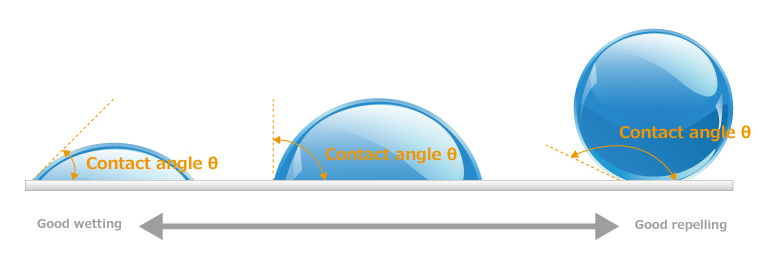
\includegraphics[scale=0.5]{4ResearchAndDevelopments/41Fibers/WettingProperty.png}
\caption{Wetting property produced by the cleaning process. \cite{WettingProperty}\label{fig:WettingProperty}}
\end{figure}


This cleaning process  was developed and carried out in the clean room of ICMOL laboratory\footnote{ICMOL, Institute of Molecular Science, is a research institute located in the Science Park of the University of Valencia.}. It consists of filling three different glass beakers, one with alkaline soap, another with millipore water\footnote{The millipore water is water in which all the ions were removed, producing a very low conductivity of it-self, on the order of $10~\mu\sievert/\cm^2$} and the last one with isopropanol. First, the fibers are rubbed for 5 minutes with alkaline soap and then placed in the first beaker for sonication for 3 minutes. Then, the fibers are cleaned with a constant flow of water for 5 minutes. Second, the fibers are placed in the second beaker for sonication for another 3 minutes. Third, the fibers are placed in the third beaker for sonication for another 3 minutes. Finally the fibers are dried with an $\ce{N_2}$ air gun and introduced inside of the prototype.

The improvement in fiber response was verified using a bundle of twenty fibers of $15~\cm$ length  that was prepared with the conditioning process described. This bundle of fibers was arranged in the setup described in section \ref{subsec:PolishingMachine}, Figure \ref{fig:BunchWith2PMTsCoincidence}, and several energy spectra were taken using different radioactive sources. Then, these fibers were cleaned with the fiber cleaning process and these measurement was repeated in the same conditions.

Two radioactive sources were used in this study, the $\ce{^{90}Sr}$ beta source, used in the polishing machine test, and the $\ce{^{137}Cs}$ gamma source, of $500~\becquerel$ activity. The results are shown in Figures \ref{fig:ResultsOfCleaningProcess}, where a shift of the spectrum to higher energies can be noticed. 

\begin{figure}
\centering
    \begin{subfigure}[b]{1\textwidth}
    \centering
    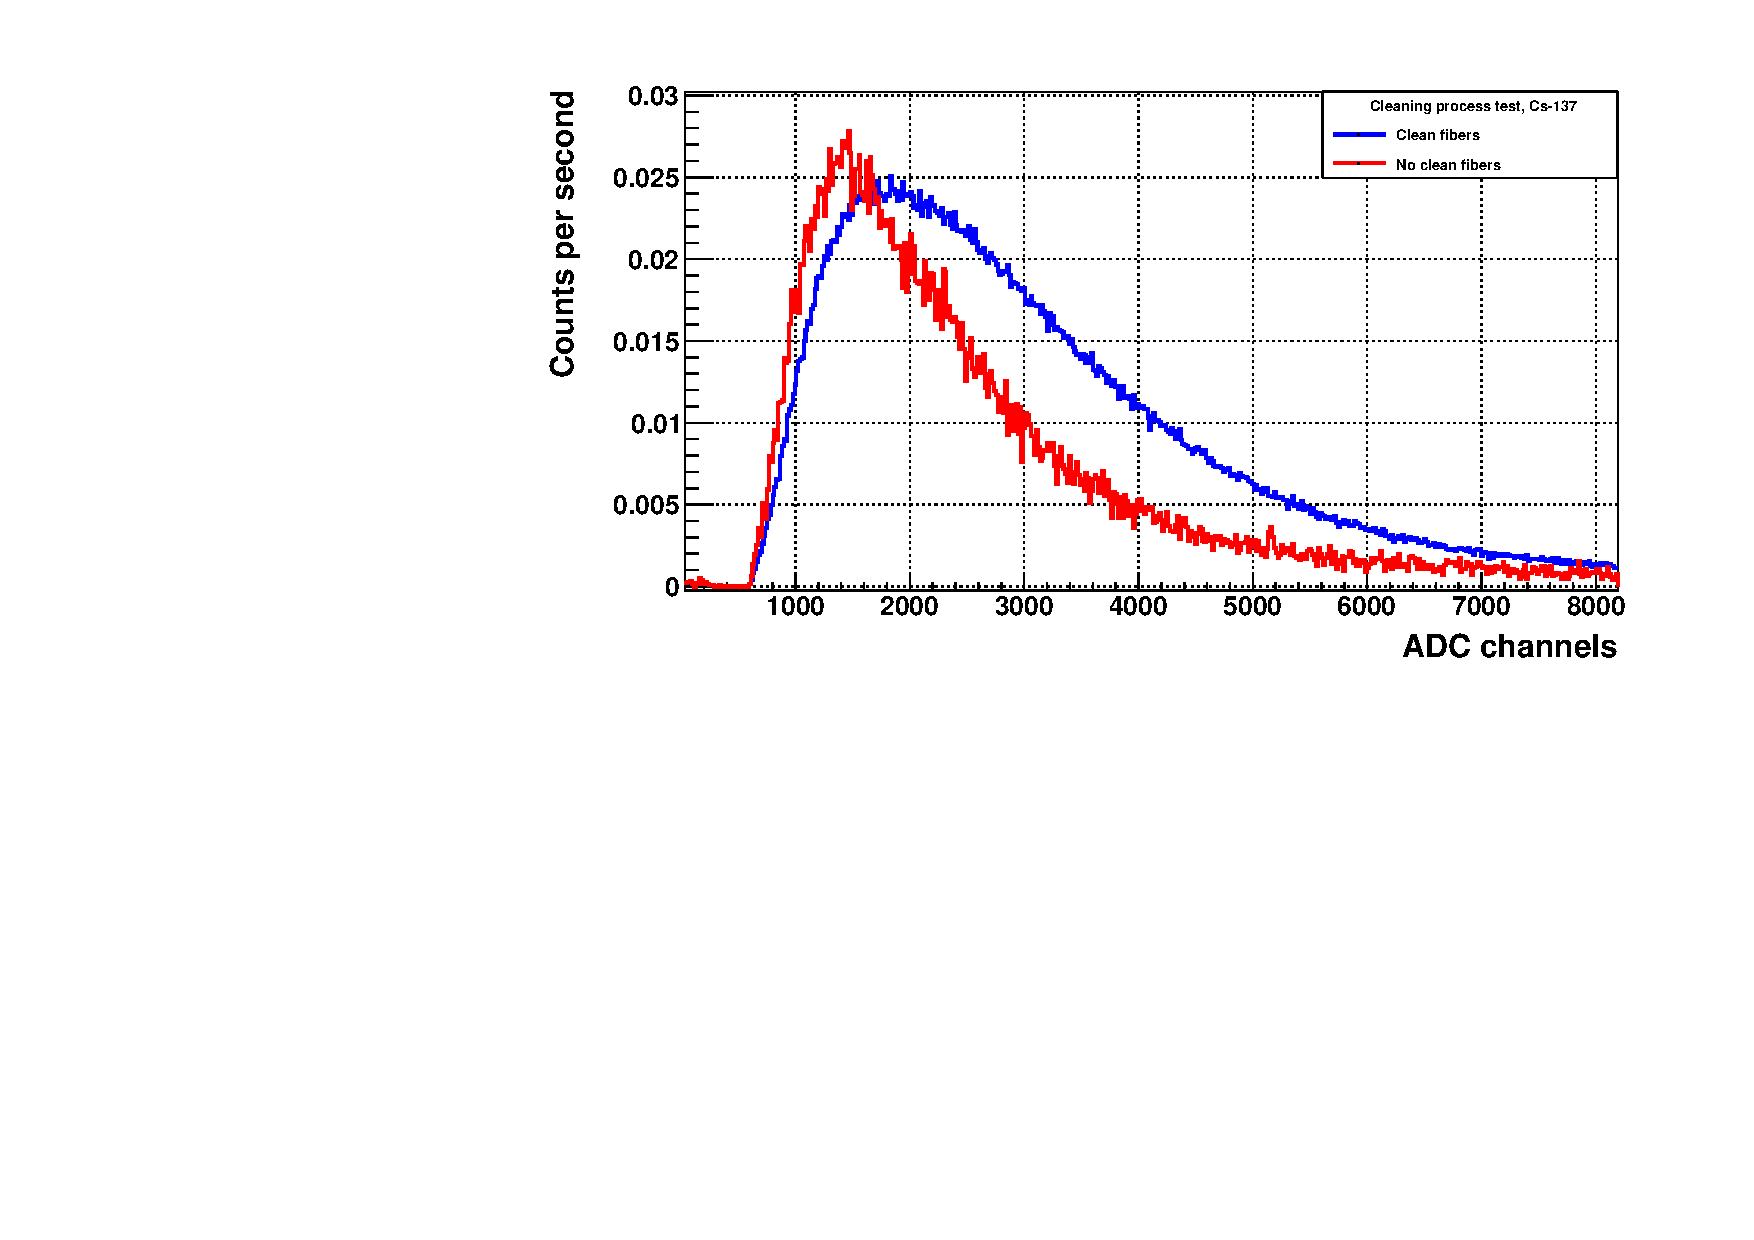
\includegraphics[width=\textwidth]{4ResearchAndDevelopments/41Fibers/Cs-137_CleaningProcess.pdf}  
    \caption{\label{subfig:EnergySpectrumCo60CleaningTest}}
    \end{subfigure}
    \hfill
    \begin{subfigure}[b]{1\textwidth}
    \centering
    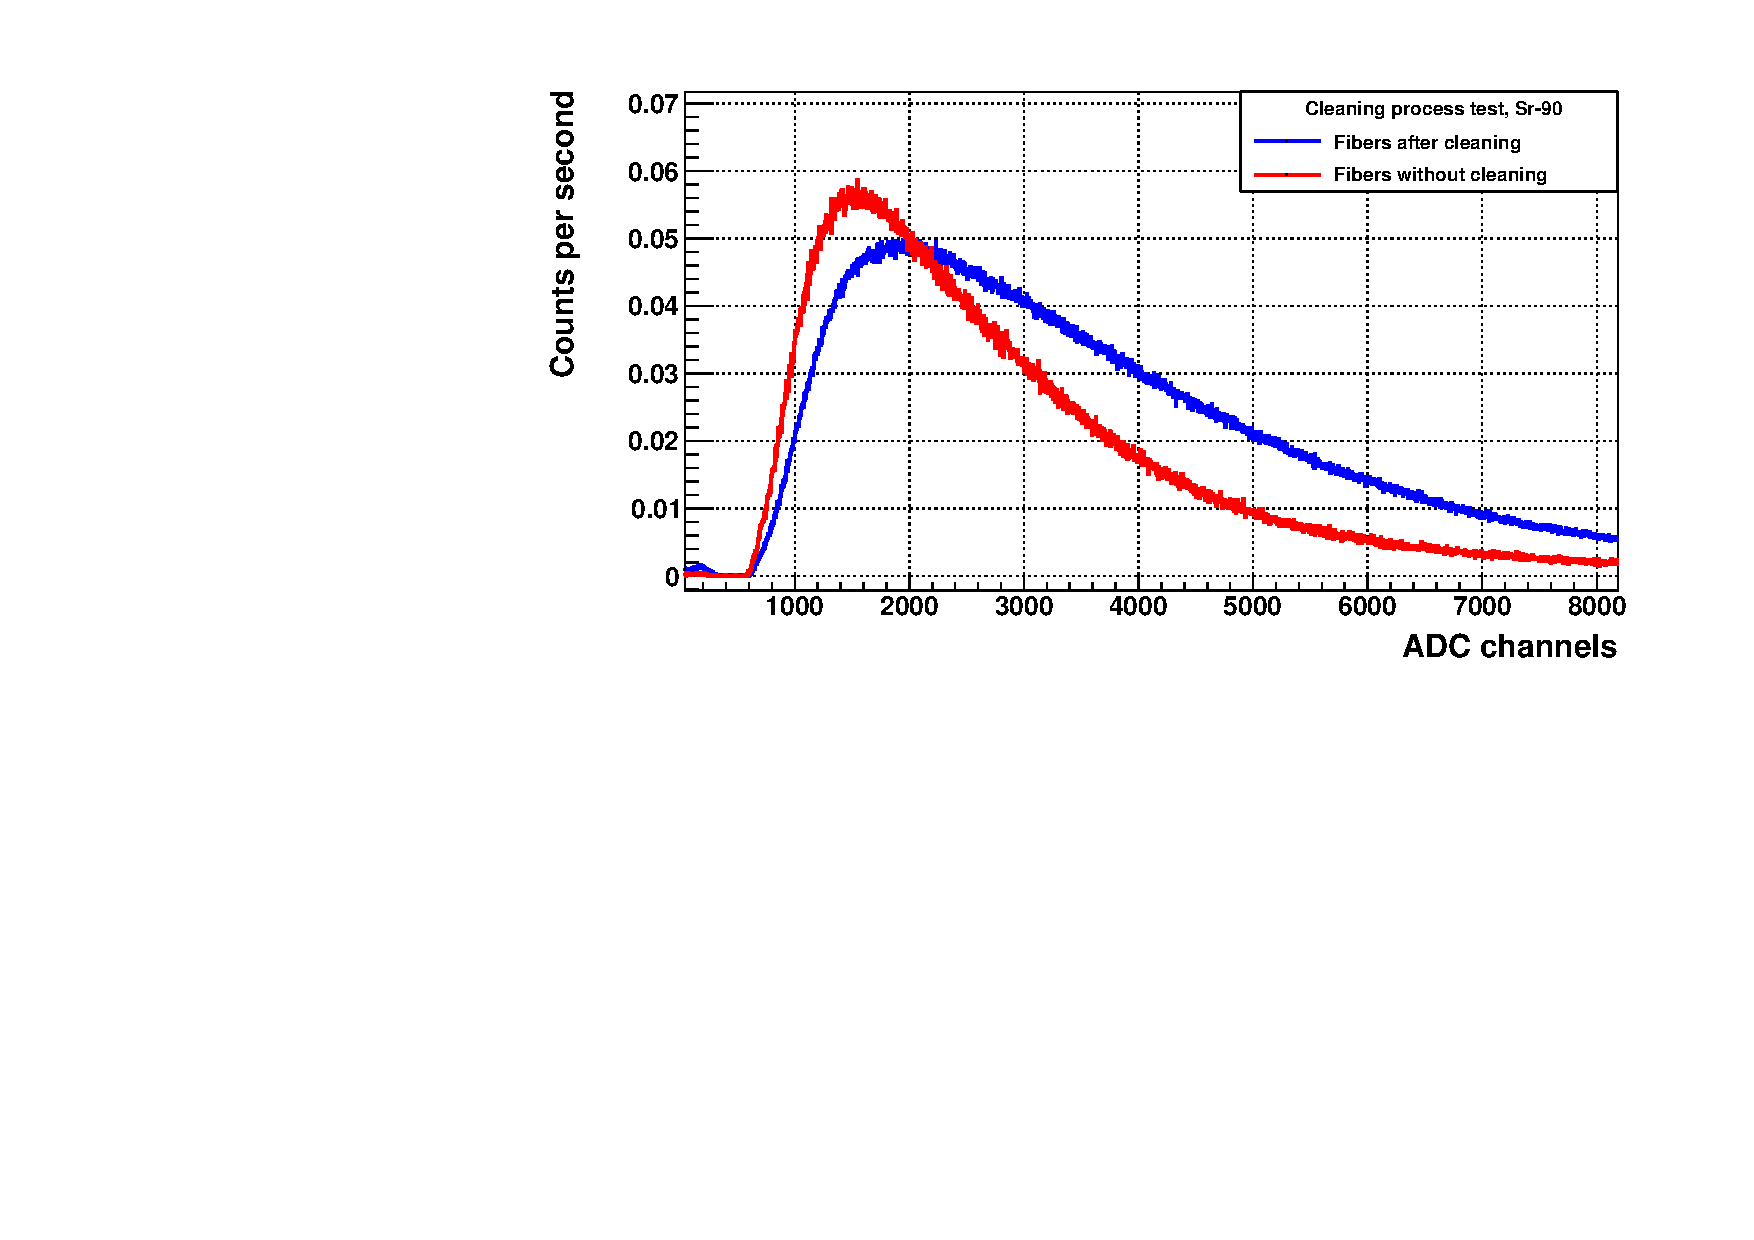
\includegraphics[width=\textwidth]{4ResearchAndDevelopments/41Fibers/Sr-90_CleaningProcess.pdf}  
    \caption{\label{subfig:EnergySpectrumSr90CleaningTest}}
    \end{subfigure}
 \caption{Energy spectra obtained before and after the cleaning process using a radioactive source of a) $\ce{^{137}Cs}$ and b) $\ce{^{90}Sr}$}
 \label{fig:ResultsOfCleaningProcess}
\end{figure}

This improvement was estimated by: 
\begin{equation}
F=\frac{A_{C}-A_{NC}}{A_{C}}
\label{eq:RelativeImprovement}
\end{equation}
where $A_{C}$ is the integral of the energy spectrum measured after the cleaning process and $A_{NC}$ is the integral of the energy spectrum measured before the cleaning process.

The F obtained is about $21\%$ for both radioactive sources. Nevertheless, it should be taken into accout that this test was carried out in air which may give somewhat different results than in water.

%$(27.73 \pm 1.6)\%$ for the gamma source and $(20.72 \pm 0.9)\%$ for the beta source so, the improvement of the photon collection efficiency of the fibers was verified using the cleaning process carried out in the clean room of ICMOL laboratories. Nevertheless, it should be taken into accout that this test was carried out in air. It could be interesting to repeat it in water to obtain more realistic conclusions since the fibers of the TRITIUM detector will be immersed in water.